%! Author = endo.axelsson
%! Date = 2023-04-19

% Preamble
\documentclass[11pt]{article}

% Packages
\usepackage{amsmath}\documentclass[11p]{article}
% Packages

\usepackage{graphicx}
\usepackage[swedish]{babel}
\usepackage[
    backend=biber,
    style=authoryear-ibid,
    sorting=ynt
]{biblatex}
\usepackage[utf8]{inputenc}
\usepackage[T1]{fontenc}
%Källor
\addbibresource{mall.bib}
\graphicspath{ {./images/} }

\title{Labrapport \\ \small Fysik 1}
\author{Endo Axelsson}
\date{\today}

\begin{document}

    \begin{titlepage}
        \begin{center}
            \vspace*{1cm}

            \Huge
            \textbf{Laboration 5}

            \vspace{0.5cm}
            \LARGE
            Ellära

            \vspace{1.5cm}

            \textbf{Endo Axelsson}

            \vfill


            Fysik 1

            \vspace{0.8cm}

            
\includegraphics[width=0.4\textwidth]{../NTI Gymnasiet_Symbol_print_svart.png}

            \Large
            Teknikprogrammet\\
            NTI Gymnasiet\\
            Umeå\\
            \today

        \end{center}
    \end{titlepage}
    \section{Syfte och frågeställning}
Räkna ut resistansen och spänningen med hjälp av mätare och se sambandet med beräkningar.

    \section{Del 1}

    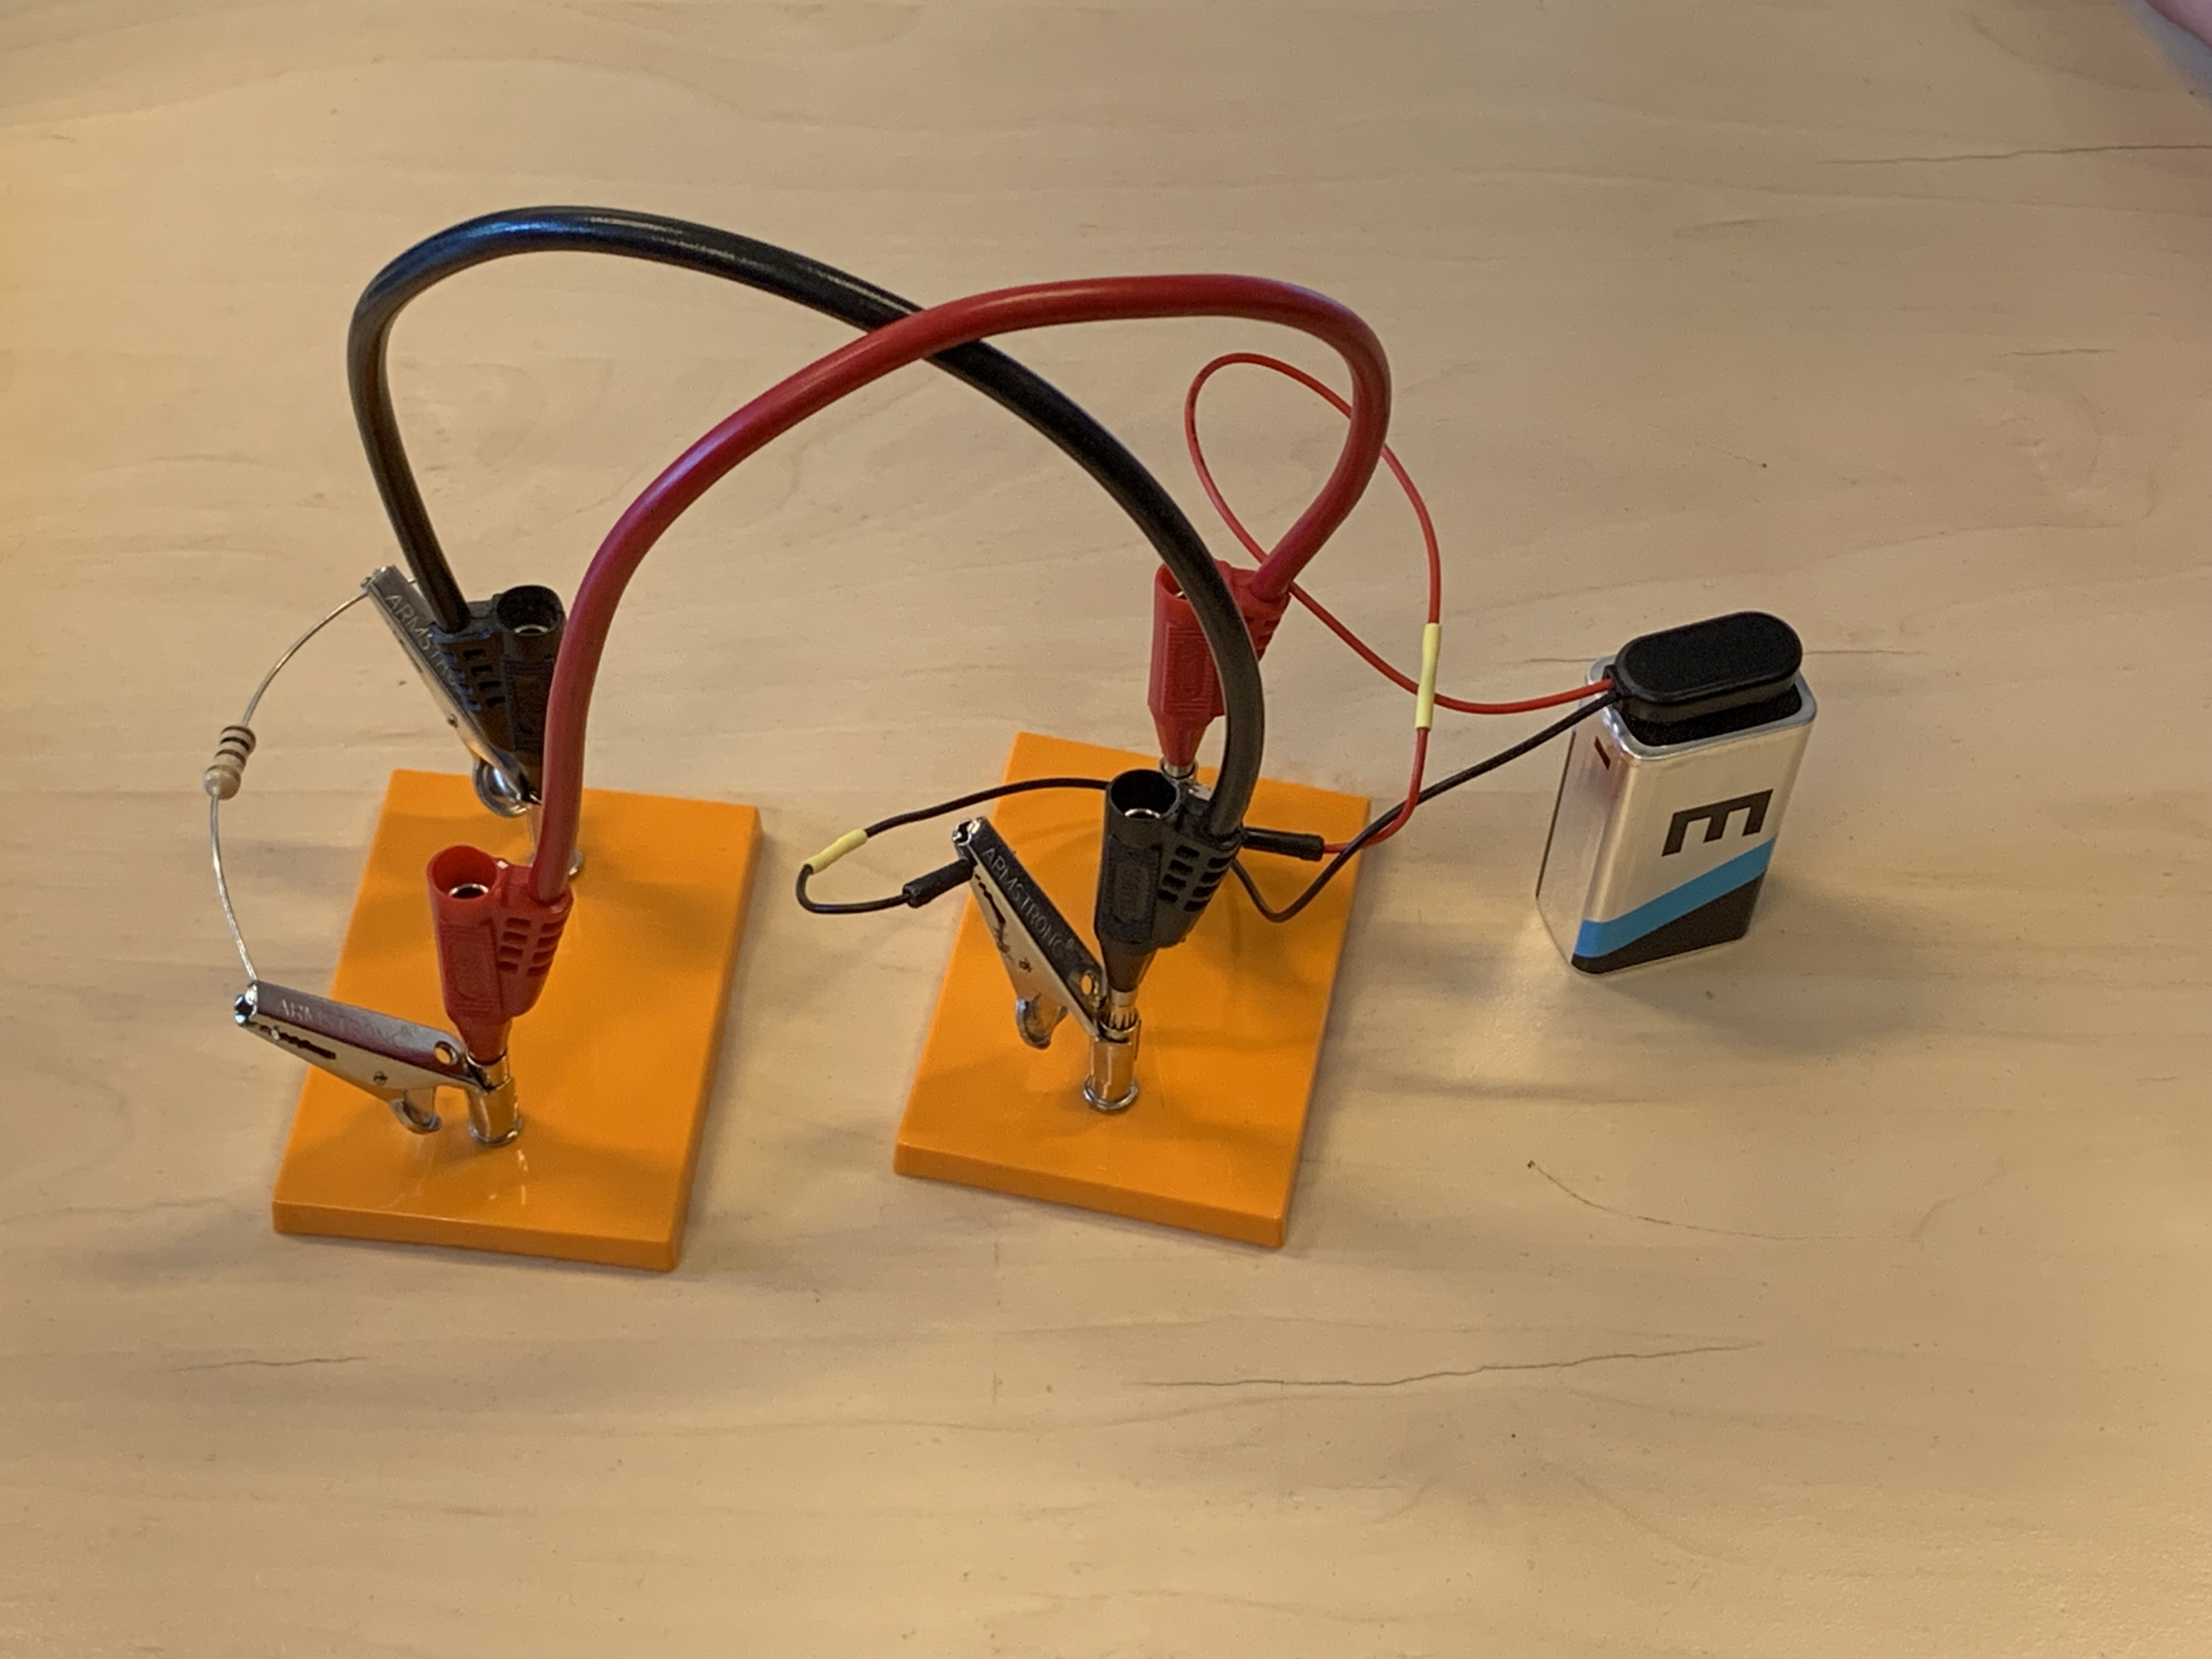
\includegraphics[width=0.6\textwidth]{../del1.jpg}

    \subsection{Material och metod}

    \begin{itemize}
        \item 1st Batteri (9V)
        \item 1st Multimeter
        \item 2st Kablar
        \item 3st kopplingsplinta
        \item 2st Krokodil klämmor
        \item 2st Motstånd
    \end{itemize}

    Vi kopplade batteriet som är 9 volt med två av krokodilklämmorna.
    På andra sidan så tog vi en resistans och klämde den mellan dem resterande två krokodilklämmorna.
    Till sist så tog vi dem två kablarna och kopplade mellan, ställde in multimeter till 20m och använde den för att få fram spänningen och strömmen.
    Anteckna ner resultat.


    \subsection{Resultat}
    Spänningen var 9V och strömmen var 0,08 ampere.
    Restistansen blev 112 ohm.

    \subsection{Analys}
    För att räkna ut resistansen så använde vi formeln \begin{equation} R = \frac{9}{0,08} \end

    där (U) är spänningen och (I) är strömmen.
    \section{Del 2}
    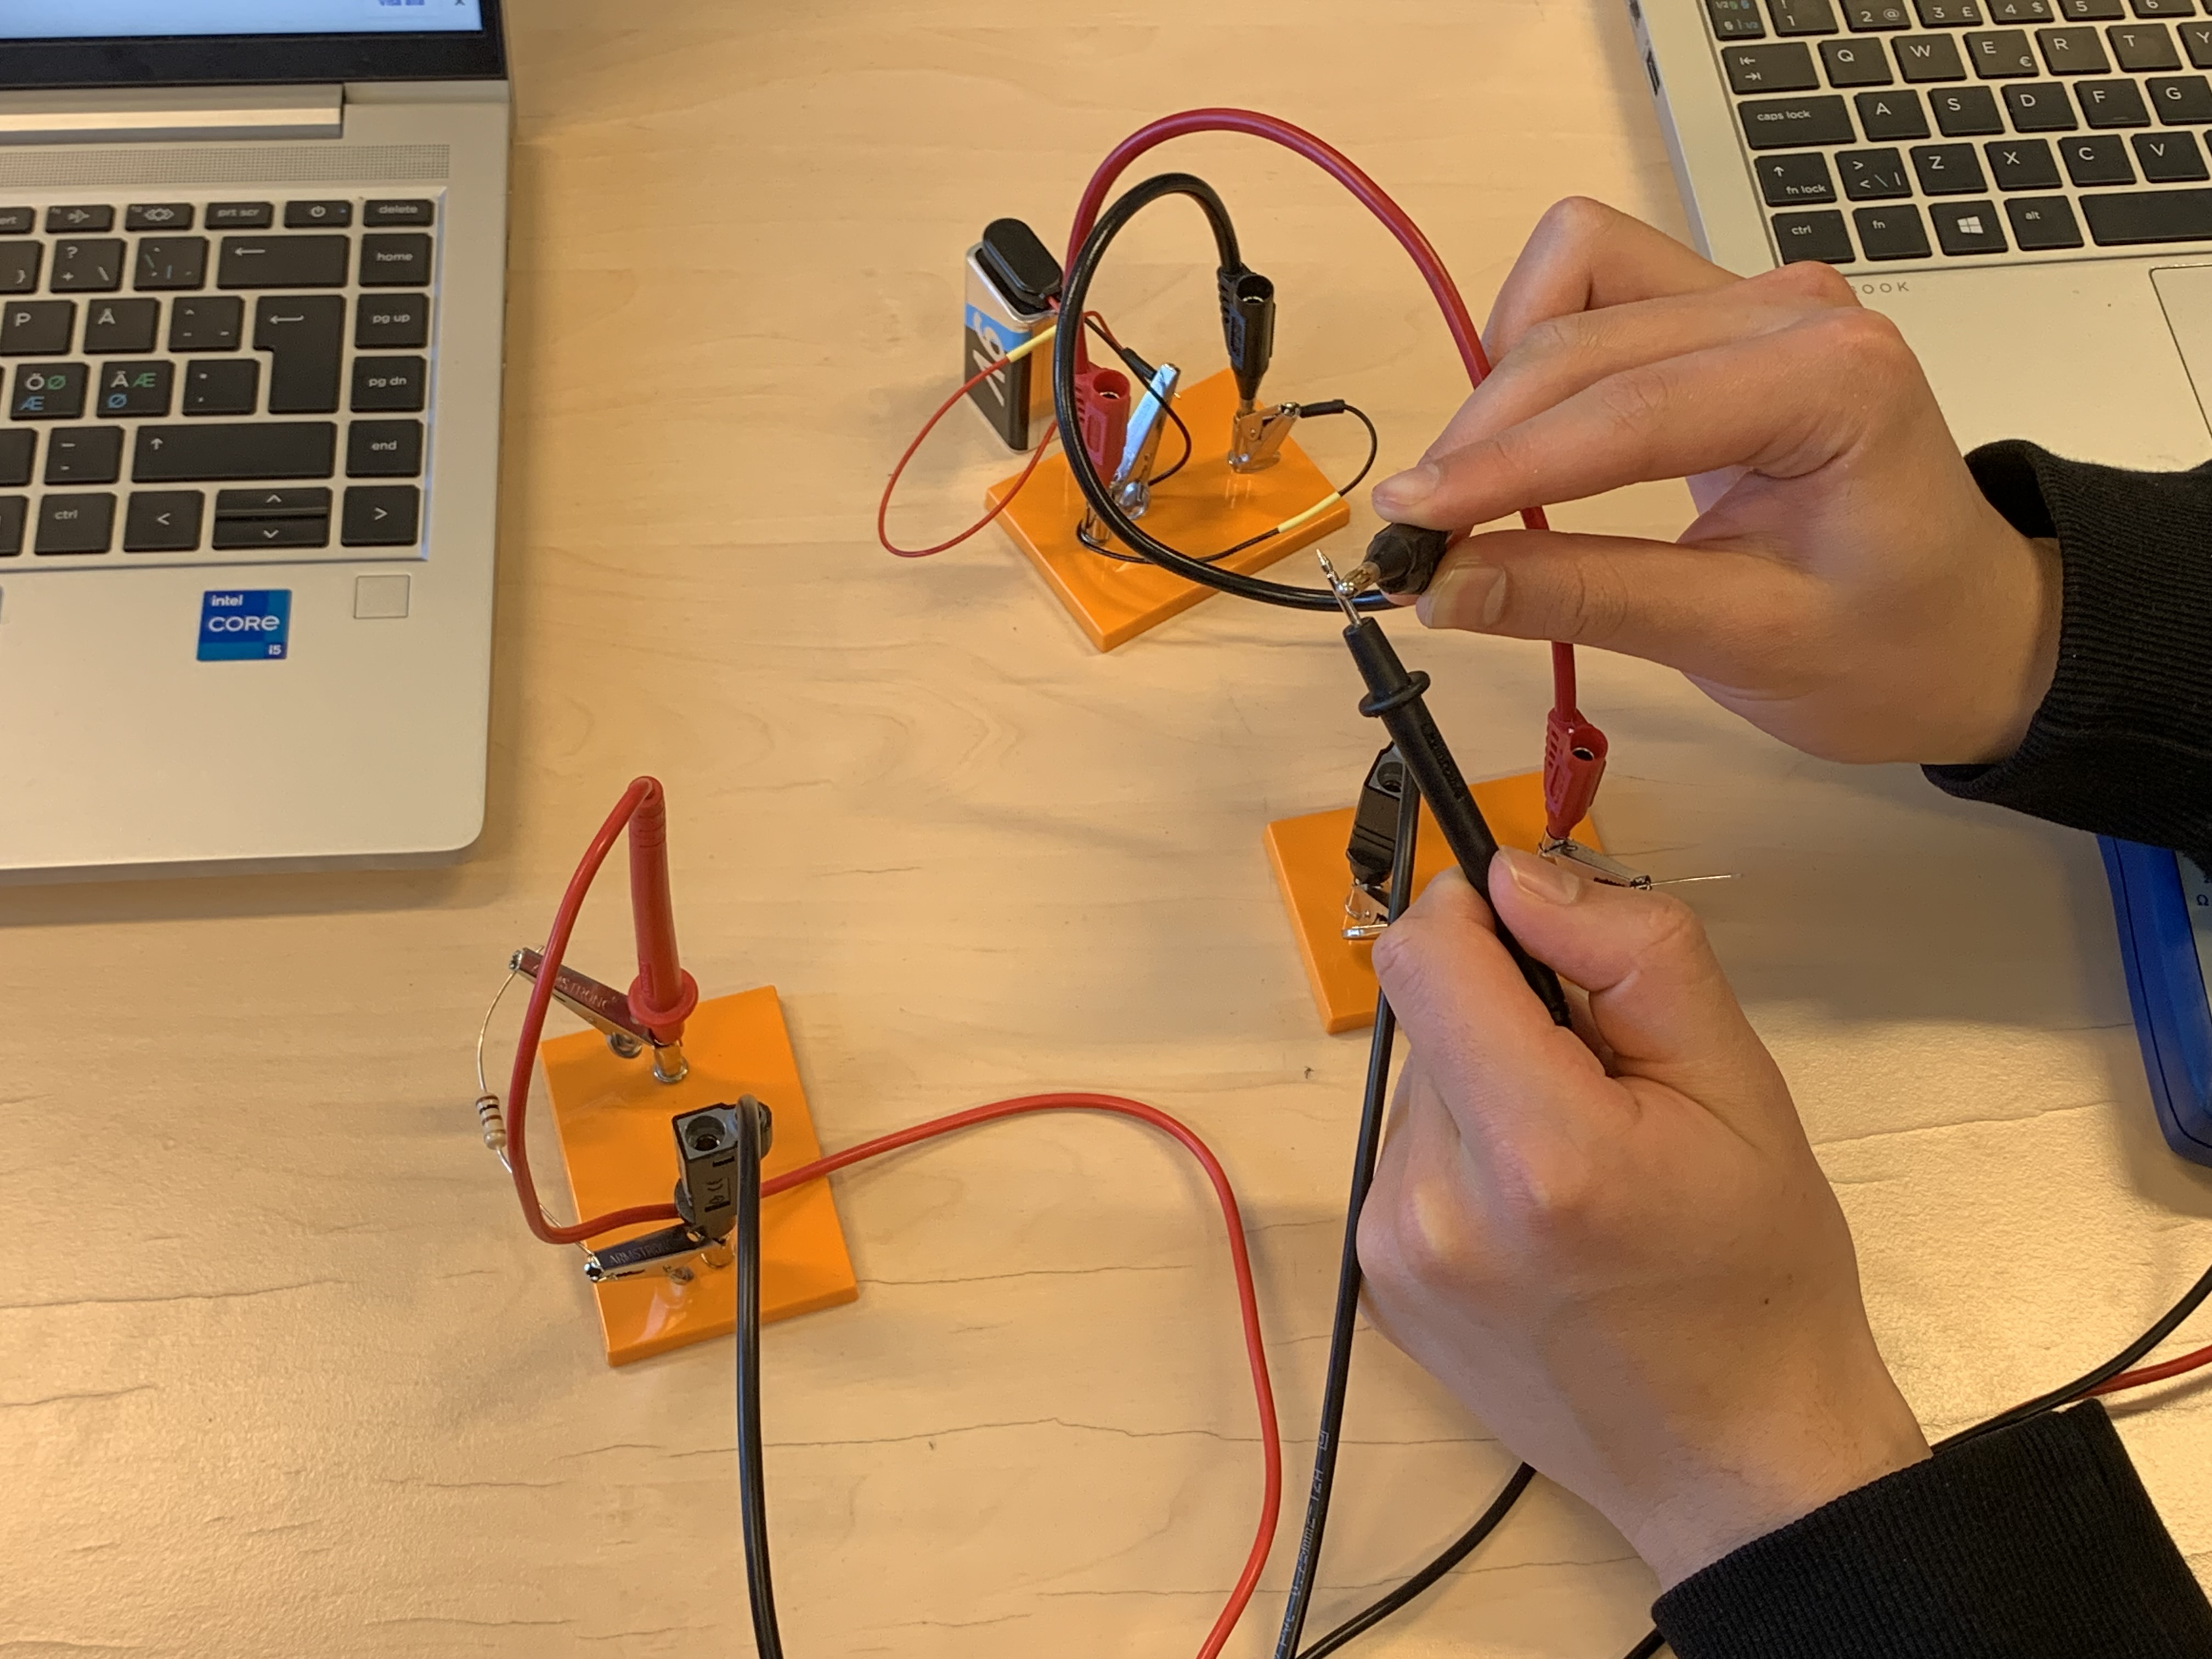
\includegraphics[width=0.6\textwidth]{../del2}
    \subsection{Material och metod}

    Samma material som del 1

    Vi hade samma struktur som i del men la till en till platta och seriekopplade.
    Andra resistansen användes nu på den nya plattan.
    Vi mätte exakt likadant.
    Vi tog multimetern och mätte både spänningen och strömmen.
    För spänningen så ställde vi in multimetern till 20V och för strömmen så använde vi 20m.

    \subsection{Resultat}

    Spänningen på ena resistansen var 4,05 volt och strömmen 0,04A
    \subsection{Analys}
    Enligt teorin så borde vi har fått spänningen 9 eftersom \begin{equation} U = 112,5 * 0,04 \end och strömmen borde då varit 0,036A med samma formel som innan: \begin{equation} I = \frac{4,05}{112,5}\end


    \section{Del 3}

    Hade inte tid.
    \subsection{Material och metod}

    Samma material som del 1


    \section{Diskussion}

    Det gick bra med metoderna.
    Hade lite småproblem då multimetern inte ville visa spänningen av någon anledning.
    Först så försökte vi koppla runt för att vi trodde att det inte fanns någon spänning men sedan så ko mvi på att det var multimetern det var fel på.
    Så vi bytte mätare och problemet var löst.
\end{document}


% Document
\begin{document}



\end{document}